\documentclass[aspectratio=169]{beamer}

\usefonttheme[stillsansserifmath]{serif}
\usepackage{graphicx}
\usepackage{amsfonts}
\usepackage{mathtools, nccmath}
\usepackage{amssymb, amsmath}
\usepackage{xspace}
\usepackage{tikz}
\usepackage{standalone}
\usepackage{euler}
\usepackage{color,xcolor}
\usepackage{fontspec}
\usepackage{nameref}
\usepackage{manfnt}
\usepackage{listings}
\usepackage{xcolor}
\usepackage{algorithm}
\usepackage[noend]{algpseudocode}
\usepackage{algorithmicx}
\usepackage{docs/style}

\usepackage{xepersian}
\settextfont{Yas}

% Persian specific
\newcommand{\itmsep}[1]{\raggedleft\setlength\itemsep{#1}}
\newcommand{\itemr}{\raggedleft\setlength\itemsep{3mm}}
\newcommand{\fn}[2]{\LR{\LTRfootnote[frame,#1]{~#2}}}
%\newcommand{\fn}[2]{{\LR{\footnote[frame,#1]{{~\LR{#2}}}}}}
\newcommand{\fnn}[1]{{\LR{\footnote[frame]{{~\LR{#1}}}}}}
\newcommand{\m}[1]{\ensuremath{\mathnormal{#1}}}
\newcommand{\mc}[1]{\ensuremath{\mathtt{#1}}}
\newcommand{\scl}{\ensuremath{\Sigma^*}\xspace}
\newcommand{\gcl}{\ensuremath{\Gamma^*}\xspace}
\newcommand{\gin}{\ensuremath{\mathnormal{\in}}\xspace}
%\newcommand{\gand}{\ensuremath{\mathnormal{\land}}\xspace}
\newcommand{\gand}{\&\&\xspace}
\newcommand{\alglr}{\LTR\ttfamily\small}
\newcommand{\st}[1]{\ensuremath{\mathnormal{\{#1\}}}\xspace}
\newcommand{\gst}[1]{\ensuremath{\mathnormal{\{\text{\texttt{#1}}\}}}\xspace}
\newcommand{\cpp}{C++\xspace}
\newcommand{\enc}[1]{\ensuremath{\mathnormal{\langle#1\rangle}}\xspace}
\newcommand{\abo}[1]{\ensuremath{\mathnormal{O(#1)}}\xspace}
\newcommand{\aso}[1]{\ensuremath{\mathnormal{o(#1)}}\xspace}
\newcommand{\aom}[1]{\ensuremath{\mathnormal{\Omega(#1)}}\xspace}
\newcommand{\ath}[1]{\ensuremath{\mathnormal{\Theta(#1)}}\xspace}
\newcommand{\dom}[2]{\ensuremath{\mathnormal{\Big[ \dfrac{#1}{#2} \Big]}}\xspace}

\newcommand{\Proc}[2]{\Statex \textbf{procedure} \textsc{#1}(#2)}
\newcommand{\Func}[2]{\Statex \textbf{function} \textsc{#1}(#2)}
\newcommand{\To}{\textbf{to}\xspace}
\newcommand{\Aand}{\textbf{and}\xspace}
\newcommand{\Aor}{\textbf{or}\xspace}



\newcommand\pro{\ensuremath{\rightarrow}\xspace}
\newcommand\der{\ensuremath{\Rightarrow}\xspace}
\newcommand\ders{\ensuremath{\stackrel{\mbox{*}}{\Rightarrow}}\xspace}
\newcommand{\dern}[1]{\ensuremath{\stackrel{\mbox{\small #1}}{\Rightarrow}}\xspace}
\newcommand\move{\ensuremath{\vdash}\xspace}
\newcommand\moves{\ensuremath{\stackrel{\small *}{\vdash}}\xspace}
\newcommand{\movesn}[1]{\ensuremath{\stackrel{\small *}{\vdash_{#1}}}\xspace}
\newcommand{\moven}[1]{\ensuremath{\mathnormal{\vdash_{#1}}}\xspace}

\newcommand{\code}[1]{{\LR{\texttt{#1}}}}
\newcommand{\txtlr}[1]{\text{\LR{#1}}}


% Abbreviations
\newcommand{\ie}{\latin{i.e.,~}}
\newcommand{\eg}{\latin{e.g.,~}}
\newcommand{\cf}{\latin{cf.~}}
\newcommand{\etal}{\latin{et al.~}}
\newcommand{\etc}{\unskip~\latin{etc.}\xspace}
\newcommand{\apriori}{\latin{a priori}}
\newcommand{\wrt}{\latin{w.r.t.~}}
%\newtheorem{theorem}{Theorem}

\newcommand\NN{\ensuremath{\mathbb{N}}\xspace}
\newcommand\RR{\ensuremath{\mathbb{R}}\xspace}
\newcommand\NNS{\ensuremath{\mathbb{N}^*}\xspace}
\newcommand\NNZ{\ensuremath{\mathbb{N}\backslash\{0\}}\xspace}
\newcommand\RRP{\ensuremath{\mathbb{R}^+}\xspace}
\newcommand\vect[1]{\ensuremath{\boldsymbol{\vec{#1}}}}
\newcommand\MP{\ensuremath{\mathcal{P}}\xspace}

\newcommand\de{\mathrel{\bullet\mkern-2.5mu{\rightarrow}}}
\newcommand\ue{\mathrel{\bullet\mkern-3mu{-}\mkern-3mu\bullet}}

\DeclareMathOperator*{\argmax}{arg\,max}
\DeclareMathOperator*{\argmin}{arg\,min}

\DeclareMathOperator{\lcm}{lcm}
\DeclareMathOperator{\Spec}{Spec}
\DeclareMathOperator{\Res}{Res}
%\DeclareMathOperator{\land}{and}

\newcommand{\fl}[1]{\ensuremath{\lfloor #1 \rfloor}}
\newcommand{\bfl}[1]{\ensuremath{\big\lfloor #1 \big\rfloor}}
\newcommand{\Bfl}[1]{\ensuremath{\Big\lfloor #1 \Big\rfloor}}
\newcommand{\bgfl}[1]{\ensuremath{\bigg\lfloor #1 \bigg\rfloor}}
\newcommand{\Bgfl}[1]{\ensuremath{\Bigg\lfloor #1 \Bigg\rfloor}}

\newcommand{\cl}[1]{\ensuremath{\lceil #1 \rceil}}
\newcommand{\bcl}[1]{\ensuremath{\big\lceil #1 \big\rceil}}
\newcommand{\Bcl}[1]{\ensuremath{\Big\lceil #1 \Big\rceil}}
\newcommand{\bgcl}[1]{\ensuremath{\bigg\lceil #1 \bigg\rceil}}
\newcommand{\Bgcl}[1]{\ensuremath{\Bigg\lceil #1 \Bigg\rceil}}

\newcommand{\mtx}[1]{\begin{pmatrix} #1 \end{pmatrix}}
\newcommand{\smtx}[1]{\begin{psmallmatrix} #1 \end{psmallmatrix}}

\definecolor{commentgreen}{RGB}{2,112,10}
\definecolor{eminence}{RGB}{108,48,130}
\definecolor{brightmaroon}{rgb}{0.76, 0.13, 0.28}
\definecolor{darkred}{rgb}{0.55, 0.0, 0.0}
\lstset {
    language=C++,
    frame=tb,
    tabsize=4,
    showstringspaces=false,
    numbers=left,
    %upquote=true,
    commentstyle=\color{commentgreen},
    keywordstyle=\color{eminence},
    stringstyle=\color{darkred},
    basicstyle=\small\ttfamily, % basic font setting
    emph={int,char,double,float,unsigned,long,short,void,bool},
    emphstyle={\color{blue}},
    %escapechar=\&,
    % keyword highlighting
    %classoffset=1, % starting new class
    %otherkeywords={>,<,.,;,-,!,=,~},
    %morekeywords={>,<,.,;,-,!,=,~},
    %keywordstyle=\color{weborange},
    %classoffset=0,
}

\makeatletter
\NewDocumentCommand{\LeftComment}{s m}{%
	\IfBooleanF{#1}{\hspace*{\ALG@thistlm}}\textcolor{commentgreen}{\(~\triangleright\) #2}}
\makeatother


\newenvironment{itemframe}[2]{
\begin{frame}[environment=itemframe]{#1}

\framesubtitle{\small \color{gray} \quad #2}
\itemize
\itemr

}{
\enditemize
\end{frame}
}

\newcommand{\centerimg}[2][.5]{
    \begin{figure}[h!]
        \centering
        \includegraphics[width=#1\textwidth]{#2}
    \end{figure}
}

\usetikzlibrary{arrows,calc}
\usetikzlibrary{positioning,shapes,chains,fit}


\tikzset{
    %Define style for boxes
    node/.style={
        circle,
        draw=black, thick,
        align=center,
    },
    ss/.style={
        circle,
        draw=black,
        align=center,
    },
    proc/.style={
        rounded corners,
        draw=black,
        align=center,
    },
    ifelse/.style={
	ellipse,
	draw=black,
	align=center,
    },
    cloudy/.style={
	cloud,
	cloud puffs=12,
	cloud ignores aspect,
	align=center,
	draw=black,
    },
    txt/.style={
        draw = none,
        align = center,
        font = \footnotesize,
    },
    coin/.style={
        rectangle,
        minimum height=1mm,
        minimum width=1cm,
        draw=black,
        fill=black!20,
        rounded corners
    },
    towercolor/.style={
        fill=black!80
    },
    towerbase/.style={
        trapezium,
        trapezium angle=75,
        trapezium stretches=true,
        towercolor,
        minimum width=7mm,
        minimum height=2mm,
    },
    tower/.style={
        rectangle,
        rounded corners,
        towercolor,
        minimum width=2mm,
        minimum height=26mm,
    },
    start-end/.style={
        draw,
        rectangle,
        rounded corners,
    },
    input/.style={ % requires library shapes.geometric
        draw,
        trapezium,
        trapezium left angle=60,
        trapezium right angle=120,
    },
    operation/.style={
        draw,
        rectangle
    },
    loop/.style={ % requires library shapes.misc
        draw,
        chamfered rectangle,
        chamfered rectangle xsep=2cm
    },
    decision/.style={ % requires library shapes.geometric
        draw,
        diamond,
        aspect=#1
    },
    decision/.default=1,
    print/.style={ % requires library shapes.symbols
        draw,
        tape,
        tape bend top=none
    },
    connection/.style={
        draw,
        circle,
        radius=5pt,
    },
    process rectangle outer width/.initial=0.15cm,
    predefined process/.style={
        rectangle,
        draw,
        append after command={
        \pgfextra{
          \draw
          ($(\tikzlastnode.north west)-(0,0.5\pgflinewidth)$)--
          ($(\tikzlastnode.north west)-(\pgfkeysvalueof{/tikz/process rectangle outer width},0.5\pgflinewidth)$)--
          ($(\tikzlastnode.south west)+(-\pgfkeysvalueof{/tikz/process rectangle outer width},+0.5\pgflinewidth)$)--
          ($(\tikzlastnode.south west)+(0,0.5\pgflinewidth)$);
          \draw
          ($(\tikzlastnode.north east)-(0,0.5\pgflinewidth)$)--
          ($(\tikzlastnode.north east)+(\pgfkeysvalueof{/tikz/process rectangle outer width},-0.5\pgflinewidth)$)--
          ($(\tikzlastnode.south east)+(\pgfkeysvalueof{/tikz/process rectangle outer width},0.5\pgflinewidth)$)--
          ($(\tikzlastnode.south east)+(0,0.5\pgflinewidth)$);
        }  
        },
        text width=#1,
        align=center
    },
    predefined process/.default=1.75cm,
    man op/.style={ % requires library shapes.geometric
        draw,
        trapezium,
        shape border rotate=180,
        text width=2cm,
        align=center,
    },
    extract/.style={
        draw,
        isosceles triangle,
        isosceles triangle apex angle=60,
        shape border rotate=90
    },
    merge/.style={
        draw,
        isosceles triangle,
        isosceles triangle apex angle=60,
        shape border rotate=-90
    },
}


\title{طراحی الگوریتم‌ها}
\author{
آرش شفیعی
}

\institute{
\\

\includegraphics[height=1.2cm]{logos/ui.png}
%\\
%دانشگاه اصفهان
}
\date{}

\begin{document}

\begin{frame}[plain]
\begin{center}
به نام خدا
\end{center}

\maketitle

%\begin{center}
%{\footnotesize arash.shafiei@gmail.com}
%\end{center}

\end{frame}
\setcounter{framenumber}{0}

%\input{docs/licence}

\raggedleft

%%%%%%%%%%%%
%\begin{frame}{فهرست مطالب}
%\begin{flushright}
%  \tableofcontents
%\end{flushright}
%\end{frame}
%%%%%%%%%%%%

%%%%%%%%%%%%
%%%%%%%%%%%%%%%%%%%%%%%%%
\section{الگوریتم‌های حریصانه}
%%%%%%%%%%%%%%%%%%%%%%%%%

\begin{frame}{‌الگوریتم‌های حریصانه}
\begin{itemize}\itemr
\item[-]
مسئله‌های بهینه‌سازی به دنبال جواب بهینه در مجموعه‌ای از جواب‌ها برای یک مسئله می‌گردند. یک جواب بهینه جوابی است که در یک معیار اندازه‌گیری بهترین باشد. برای مثال یک جواب بهینه می‌تواند کوچک‌ترین، بزرگ‌ترین، کوتاهترین، بلندترین و غیره باشد.
\item[-]
برنامه‌ریزی پویا یکی از روش‌ها برای حل مسئله‌های بهینه‌سازی است.
\item[-]
الگوریتم‌های حریصانه
\fn{1}{greedy algorithms}
دسته‌ای دیگر از الگوریتم‌ها برای حل مسئله‌های بهینه‌سازی هستند.
\end{itemize}
\end{frame}


\begin{frame}{‌الگوریتم‌های حریصانه}
\begin{itemize}\itemr
\item[-]
فرض کنید می‌خواهیم در مدت
\m{n}
روز به بیشترین دارایی ممکن دست پیدا کنیم.
برای این کار کافی است که در هر روز بیشترین دارایی ممکن را کسب کنیم.
بنابراین برای به دست آوردن بیشترین دارایی در مدت
\m{n}
روز باید در روز اول بیشترین دارایی را کسب کنیم و زیر مسئله‌ای که باید در گام بعد حل شود این است که چگونه در مدت
\m{n-1}
روز بیشترین دارایی را کسب کنیم.
پس در هر روز یک انتخاب حریصانه انجام می‌دهیم و آن انتخاب، کسب بیشترین دارایی در همان روز است. می‌دانیم که با این انتخاب حریصانه در مدت
\m{n}
روز بیشترین دارایی را کسب خواهیم کرد.
\item[-]
یک الگوریتم حریصانه مسئله را از بالا به پایین حل می‌کند. برای حل یک مسئله به روش حریصانه در هر گام یک انتخاب بهینه انجام می‌شود و از یک مسئله یک زیرمسئله به دست می‌آید.
این فرایند ادامه پیدا می‌کند تا زیرمسئله‌ای باقی نماند. در پایان جواب مسئله مجموعهٔ همهٔ انتخاب‌های بهینه است.
به عبارت دیگر در هر گام یک انتخاب حریصانه برای به دست آوردن جواب بهینه صورت می‌گیرد و در پایان مجموعهٔ همهٔ انتخاب‌های حریصانه جواب مسئله است.
% و در هر گام الگوریتم انتخاب‌هایی می‌کند تا به پاسخ بهینه برسد. در الگوریتم‌های حریصانه 
% در هر گام، الگوریتم بهینه‌ترین انتخاب را انجام می‌دهد به این امید که در پایان جواب بهینه به دست آید.
%\item[-]
%الگوریتم‌های حریصانه تنها در برخی از مسائل با ویژگی‌های خاص به پاسخ بهینه دست می‌یابند.
\end{itemize}
\end{frame}


\begin{frame}{‌الگوریتم‌های حریصانه}
\begin{itemize}\itemr
\item[-]
تنها برخی از مسئله‌های بهینه‌سازی را می‌توان به روش حریصانه حل کرد.
\item[-]
برای مثال مسئله درخت جستجوی دودویی بهینه را در نظر بگیرید. اگر در هر گام برای ساختن درخت جستجوی دودویی بهینه از بین همهٔ کلیدها، کلیدی را به عنوان ریشه در نظر بگیریم که بیشترین احتمال وقوع را داشته باشد، درخت به دست آمده الزاما بهینه نیست.
\item[-]
همانطور که مشاهده کردیم ریشهٔ یک درخت جستجوی دودویی بهینه ممکن است کلیدی باشد که بیشترین احتمال وقوع را نداشته باشد.
%\item[-]
%در صورتی یک مسئله را می‌توان به روش حریصانه حل کرد که پس از نوشتن رابطه بازگشتی، تنها یک زیرمسئله جواب مسئله باشد.
\end{itemize}
\end{frame}

\begin{frame}{‌مسئله انتخاب فعالیت‌ها}
\begin{itemize}\itemr
\item[-]
در مسئله انتخاب فعالیت‌ها
\fn{1}{activity selection problem}
، تعدادی فعالیت به طور همزمان می‌خواهند انجام شوند به طوری‌که این فعالیت‌ها از یک منبع مشترک استفاده می‌کنند و این منبع مشترک نمی‌تواند به طور همزمان توسط فعالیت‌ها استفاده شود. می‌خواهیم مجموعه‌ای از فعالیت‌ها را انتخاب کنیم، به طوری که بیشترین تعداد فعالیت‌ها بتوانند اجرا شوند.
\item[-]
فرض کنید شما مسئول زمانبندی یک اتاق کنفرانس هستید. به شما مجموعهٔ
\m{S = \{a_1,a_2, \cdots, a_n \}}
شامل n فعالیت داده شده است که می‌خواهند اتاق کنفرانس را رزرو کنند. در این اتاق در یک زمان تنها یک فعالیت می‌تواند صورت بگیرد.
\end{itemize}
\end{frame}


\begin{frame}{‌مسئله انتخاب فعالیت‌ها}
\begin{itemize}\itemr
\item[-]
هر فعالیت
\m{a_i}
یک زمان شروع
\fn{1}{state time}
\m{s_i}
و یک زمان پایان
\fn{2}{finish time}
\m{f_i}
دارد به طوری‌که
\m{0 \leqslant s_i < f_i < \infty}.
اگر فعالیت
\m{a_i}
انتخاب شود، آنگاه این فعالیت می‌تواند در بازهٔ زمانی
\m{[s_i,f_i)}
انجام شود. دو فعالیت
\m{a_i}
و
\m{a_j}
سازگار
\fn{3}{compatible}
گفته می‌شوند اگر بازه‌های زمانی
\m{[s_i,f_i)}
و
\m{[s_j,f_j)}
تداخل نداشته باشند. دو فعالیت تداخل ندارند اگر
\m{s_i \geqslant f_j}
یا
\m{s_j \geqslant f_i}
. در مسئلهٔ انتخاب فعالیت‌ها، هدف این است که بیشترین تعداد فعالیت‌های سازگار از یک مجموعهٔ فعالیت‌ها انتخاب شوند.
\item[-]
فرض می‌کنیم فعالیت‌ها بر اساس زمان پایان‌شان مرتب شده‌اند. به عبارت دیگر :
\begin{align*}
\m{f_1 \leqslant f_2 \leqslant f_3 \leqslant \cdots \leqslant f_{n-1} \leqslant f_n}
\end{align*}
\end{itemize}
\end{frame}


\begin{frame}{‌مسئله انتخاب فعالیت‌ها}
\begin{itemize}\itemr
\item[-]
برای مثال مجموعه‌ای از فعالیت‌ها در جدول زیر را در نظر بگیرید.
\begin{figure}
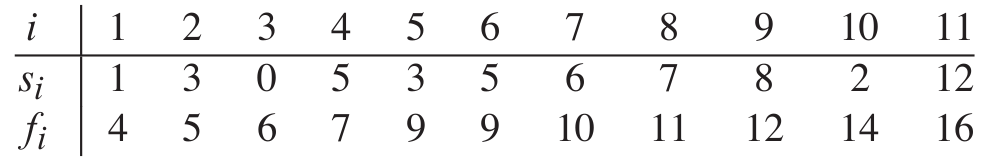
\includegraphics[width=0.7\textwidth]{figs/chap05/activity-example}
\end{figure}
\item[-]
مجموعهٔ
\m{\{a_3,a_9,a_{11}\}}
مجموعه‌ای از فعالیت‌های سازگار است ولی بزرگ‌ترین مجموعهٔ فعالیت‌های سازگار نیست چراکه
\m{\{a_1,a_4,a_8,a_{11}\}}
تعداد بیشتری فعالیت را شامل می‌شود.
همچنین مجموعهٔ
\m{\{a_2,a_4,a_9,a_{11}\}}
تعداد چهار فعالیت را شامل می‌شود.
\end{itemize}
\end{frame}



\begin{frame}{‌مسئله انتخاب فعالیت‌ها}
\begin{itemize}\itemr
\item[-]
در اینجا ابتدا سعی می‌کنیم مسئلهٔ انتخاب فعالیت‌ها را توسط برنامه‌ریزی پویا حل کنیم.
\item[-]
 فرض کنید
\m{S_{ij}}
مجموعه‌ای از فعالیت‌ها باشد که پس از اتمام فعالیت
\m{a_i}
آغاز
و قبل از شروع فعالیت
\m{a_j}
تمام می‌شوند.
فرض کنید می‌خواهیم حداکثر فعالیت‌های سازگار
\m{S_{ij}}
را پیدا کنیم و فرض کنید
\m{A_{ij}}
مجموعه‌ای است که شامل حداکثر تعداد فعالیت‌های سازگار از مجموعهٔ
\m{S_{ij}}
است.
\item[-]
حال فرض کنید
\m{a_k}
یکی از فعالیت‌ها در مجموعهٔ
\m{A_{ij}}
است. در اینجا دو زیر مسئله داریم : مسئلهٔ یافتن حداکثر فعالیت‌های سازگار در
\m{S_{ik}}
(که شامل فعالیت‌هایی می‌شود که پس از اتمام
\m{a_i}
آغاز
و قبل از شروع
\m{a_k}
پایان می‌یابند) و مسئلهٔ یافتن حداکثر فعالیت‌های سازگار در
\m{S_{kj}}
(که شامل فعالیت‌هایی می‌شود که پس از اتمام
\m{a_k}
آغاز
و قبل از شروع
\m{a_j}
پایان می‌یابند).
\end{itemize}
\end{frame}

\begin{frame}{‌مسئله انتخاب فعالیت‌ها}
\begin{itemize}\itemr
\item[-]
در گام اول باید ثابت کنیم مسئله دارای زیرساختار بهینه است.
\item[-]
 فرض کنید
\m{a_k}
در مجموعهٔ جواب
\m{A_{ij}}
است.
حال فرض کنید
\m{A_{ik} = A_{ij}\cap S_{ik}}
و
\m{A_{kj} = A_{ij}\cap S_{kj}},
بنابراین
\m{A_{ik}}
شامل فعالیت‌هایی در
\m{A_{ij}}
می‌شود که قبل از شروع
\m{a_k}
پایان می‌یابند و
\m{A_{kj}}
شامل فعالیت‌هایی در
\m{A_{ij}}
می‌شود که پس از اتمام
\m{a_k}
شروع می‌شوند.
\item[-]
اگر
\m{a_k}
در 
\m{A_{ij}}
باشد، الزاما
\m{A_{ik}}
جواب مسئله
\m{S_{ik}}
و
\m{A_{kj}}
جواب مسئله
\m{S_{kj}}
است.
\item[-]
با استفاده از برهان خلف می‌توانیم اثبات کنیم پاسخ بهینه برای
\m{S_{ij}}
شامل پاسخ بهینه برای دو زیر مسئله
\m{S_{ik}}
و
\m{S_{kj}}
می‌شود. اگر می‌توانستیم مجموعه
\m{A'_{kj}}
از حداکثر فعالیت‌های سازگار
\m{S_{kj}}
را پیدا کنیم به طوری‌که
\m{|A'_{kj}| > |A_{kj}|}
آنگاه می‌توانستیم از
\m{A'_{kj}}
به جای
\m{A_{kj}}
در زیر مسئلهٔ
\m{S_{ij}}
استفاده کنیم و بنابراین داشتیم :\\
\m{|A_{ik}| + |A'_{kj}| + 1 > |A_{ik}| + |A_{kj}| + 1 = |A_{ij}|}
که با فرض اینکه
\m{A_{ij}}
جواب بهینه است در تناقض است.
\end{itemize}
\end{frame}

\begin{frame}{‌مسئله انتخاب فعالیت‌ها}
\begin{itemize}\itemr
\item[-]
طبق تعریف می‌دانیم
حداکثر تعداد فعالیت‌ها در 
\m{S_{ik}}
برابر است با
\m{A_{ik}}
و
حداکثر تعداد فعالیت‌ها در 
\m{S_{kj}}
برابر است با
\m{A_{kj}} .
\item[-]
بنابراین داریم
\m{A_{ij} = A_{ik}\cup \{a_k \} \cup A_{kj}}
و در نتیجه
\m{|A_{ij}| = |A_{ik}| + |A_{kj}| + 1}.
\end{itemize}
\end{frame}


\begin{frame}{‌مسئله انتخاب فعالیت‌ها}
\begin{itemize}\itemr
\item[-]
فرض کنید اندازه مجموعه جواب بهینه برای
\m{S_{ij}}
را با
\m{c[i,j]}
نشان دهیم، 
بنابراین 
\m{|A_{ij}| = c[i,j]} .
\item[-]
آنگاه می توانیم بنویسیم :
\m{c[i,j] = c[i,k] + c[k,j] + 1}.
\item[-]
از آنجایی که نمی‌دانیم به ازای کدام
\m{a_k}
جواب بهینه به‌دست می‌آید، بنابراین باید همهٔ
\m{a_k}
ها را در نظر بگیریم تا جواب بهینه را به دست آوریم.
\begin{align*}
\m{c[i,j] = } \left\{ \begin{array}{lr}
					\m{0} & \m{S_{ij} = \emptyset}~~\text{اگر}\\
					\m{\max \{c[i,k] + c[k,j] + 1 : a_k \in S_{ij} \}} & \m{S_{ij} \neq \emptyset}~~\text{اگر}
					\end{array}\right.
\end{align*}
\item[-]
سپس می‌توانیم این مسئله را به روش برنامه‌ریزی پویا حل کنیم.
%\item[-]
%مشاهده خواهیم کرد که به جای چند انتخاب برای زیر مسئله‌های بهینه، در این مسئله همیشه در هنگام استفاده از برنامه‌ریزی پویا، تنها یک زیرمسئلهٔ بهینه وجود دارد. انتخاب این زیرمسئلهٔ بهینه همان انتخاب حریصانه است. درواقع با یک انتخاب حریصانه در هرگام از الگوریتم در نهایت به جواب بهینه دست پیدا می‌کنیم.
\end{itemize}
\end{frame}


\begin{frame}{‌مسئله انتخاب فعالیت‌ها}
\begin{itemize}\itemr
\item[-]
می‌توانیم رابطهٔ به دست آمده را ساده‌تر کنیم.
\item[-]
در مجموعهٔ
\m{S_{ij}}
همیشه یکی از عناصر به عنوان اولین عنصری است که در مجموعهٔ
\m{A_{ij}}
قرار می‌گیرد.
\item[-]
می‌خواهیم اولین عنصر از مجموعهٔ 
\m{S_{ij}}
که در مجموعهٔ 
\m{A_{ij}}
قرار می‌گیرد را انتخاب کنیم.
\item[-]
پس صورت مسئله را تغییر می‌دهیم.
\end{itemize}
\end{frame}


\begin{frame}{‌مسئله انتخاب فعالیت‌ها}
\begin{itemize}\itemr
\item[-]
فرض کنید
\m{S_k = \{a_i  \in S : s_i \geqslant f_k \}}
مجموعه‌ای از فعالیت‌ها باشد که پس از اتمام
\m{a_k}
آغاز می‌شوند.
\item[-]
اولین فعالیت در 
\m{S_k}
که در بزرگترین مجموعهٔ سازگار فعالیت‌ها قرار می‌گیرد کدام است؟
\end{itemize}
\end{frame}

\iffalse
\begin{frame}{‌مسئله انتخاب فعالیت‌ها}
\begin{itemize}\itemr
\item[-]
انتخاب حریصانه
\m{a_1}
اولین فعالیتی است که
انتخاب می‌شود و پس از آن
\m{S_1}
زیر مسئلهٔ بعدی است که باید حل شود.
\item[-]
بنابراین اگر
\m{a_1}
متعلق به مجموعهٔ جواب بهینه باشد، آنگاه مجموعه جواب بهینه برای کل مسئله برابر است با
\m{a_1}
 و تمام فعالیت‌هایی که به جواب زیر مسئلهٔ
\m{S_1}
تعلق دارند.
\item[-]
این راه‌حل را به طور شهودی به دست آوردیم. حال باید اثبات کنیم که این راه‌حل درست است.
\end{itemize}
\end{frame}
\fi

\begin{frame}{‌مسئله انتخاب فعالیت‌ها}
\begin{itemize}\itemr
\item[-]
قضیه : فرض کنید
\m{S_k}
مجموعه‌ای غیر تهی از فعالیت‌هاست و
\m{a_m}
فعالیتی است در
\m{S_k}
که کوچک‌ترین زمان پایان را دارد. آنگاه
\m{a_m}
در بزرگ‌ترین مجموعهٔ فعالیت‌های سازگار
\m{S_k}
قرار دارد.
\item[-]
اثبات : فرض کنید
\m{A_k}
بزرگ‌ترین مجموعهٔ فعالیت‌های سازگار
\m{S_k}
باشد و
\m{a_j}
فعالیتی در
\m{A_k}
باشد که کوچکترین زمان پایان را دارد. اگر
\m{a_j = a_m}
باشد به نتیجه مطلوب رسیده‌ایم یعنی در واقع
\m{a_m}
متعلق به بزرگ‌ترین مجموعهٔ فعالیت‌های سازگار
\m{S_k}
است.
\item[-]
حال فرض کنیم
\m{a_j \neq a_m}
باشد. مجموعهٔ
\m{A'_k = (A_k - \{a_j\}) \cup \{a_m\}}
را به عنوان مجموعه‌ای که شامل
\m{a_j}
نیست ولی
\m{a_m}
را شامل می‌شود در نظر بگیرید. فعالیت‌های
\m{A'_k}
سازگار هستند، زیرا فعالیت‌های
\m{A_k}
سازگار هستند،
و
\m{a_j}
اولین فعالیت در
\m{A_k}
است که به اتمام می‌رسد و
\m{f_m \leqslant f_j}.
از آنجایی که
\m{|A'_k| = |A_k|}
، نتیجه می‌گیریم که
\m{A'_k}
نیز بزرگ‌ترین مجموعه فعالیت‌های سازگار
\m{S_k}
است که
\m{a_m}
را نیز شامل می‌شود.
\end{itemize}
\end{frame}



\begin{frame}{‌مسئله انتخاب فعالیت‌ها}
\begin{itemize}\itemr
\item[-]
فرض کنید اندازه مجموعه جواب بهینه برای
\m{S_{k}}
را با
\m{c[k]}
نشان دهیم، 
بنابراین 
\m{|A_{k}| = c[k]} .
\item[-]
اگر اولین عضو مجموعهٔ
\m{S_k}
فعالیت
\m{a_m}
باشد، طبق قضیه قبل
\m{a_m}
در
\m{A_k}
است.
  مجموعه فعالیت‌های باقیمانده
\m{S_{m}}
است و در اینصورت
می توانیم بنویسیم :
\m{c[k] = 1 + c[m]}.
\item[-]
بنابراین می‌توانیم بنویسیم:
\begin{align*}
\m{c[k] = } \left\{ \begin{array}{lr}
					\m{0} & \m{S_{k} = \emptyset}~~\text{اگر}\\
					\m{1 + c[m]} & \text{باشد.}~\m{S_k}~\text{اولین عضو}~\m{a_m}~\text{و}~\m{S_{k} \neq \emptyset}~~\text{اگر}
					\end{array}\right.
\end{align*}
\item[-]
در اینجا یک رابطهٔ بازگشتی به دست آوردیم که همیشه تنها یک انتخاب بهینه در آن وجود دارد.
در صورتی که بتوانیم چنین رابطهٔ بازگشتی برای یک مسئله پیدا کنیم، که در آن همیشه یک انتخاب بهینه وجود داشته باشد، می‌توانیم مسئله را با استفاده از روش حریصانه حل کنیم.
%\item[-]
%مشاهده خواهیم کرد که به جای چند انتخاب برای زیر مسئله‌های بهینه، در این مسئله همیشه در هنگام استفاده از برنامه‌ریزی پویا، تنها یک زیرمسئلهٔ بهینه وجود دارد. انتخاب این زیرمسئلهٔ بهینه همان انتخاب حریصانه است. درواقع با یک انتخاب حریصانه در هرگام از الگوریتم در نهایت به جواب بهینه دست پیدا می‌کنیم.
\end{itemize}
\end{frame}


\iffalse
\begin{frame}{‌مسئله انتخاب فعالیت‌ها}
\begin{itemize}\itemr
\item[-]
اما این مسئله را می‌توانیم به روشی ساده‌تر نیز حل کنیم. به طور شهودی می‌توانیم حدس بزنیم که باید فعالیت‌هایی را انتخاب کنیم که امکان انتخاب حداکثر تعداد فعالیت‌ها را به ما بدهند، بنابراین به طور شهودی می‌توانیم حدس بزنیم باید فعالیتی ابتدا تمام شود که زمان پایان آن زودتر باشد تا تعداد بیشتری فعالیت بتوانند به عنوان فعالیت بعدی انتخاب شوند.
\item[-]
به عبارت دیگر از آنجایی که فعالیت‌ها به ترتیب بر اساس زمان پایان‌شان مرتب شده‌اند و در ابتدا فعالیتی انتخاب می‌شود که زمان پایان آن از همه زودتر باشد، بنابراین فعالیت
\m{a_1}
انتخاب می‌شود. سپس فعالیتی انتخاب شود که زمان شروع آن پس از زمان اتمام
\m{a_1}
باشد تا با
\m{a_1}
تداخل نداشته باشد و ضمنا زمان پایان آن از بقیه فعالیت‌های ممکن کمتر باشد. پس اولین فعالیت پس از
\m{a_1}
که زمان شروع آن پس از اتمام
\m{a_1}
است انتخاب می‌شود.
\end{itemize}
\end{frame}
\fi

\iffalse
\begin{frame}{‌مسئله انتخاب فعالیت‌ها}
\begin{itemize}\itemr
\item[-]
گرچه توانستیم مسئله انتخاب فعالیت‌ها را با استفاده از برنامه‌ریزی پویا حل کنیم، ولی با استفاده از قضیه قبل می‌توانیم این مسئله را به روشی دیگر نیز حل کنیم.
\end{itemize}
\end{frame}
\fi


\begin{frame}{‌مسئله انتخاب فعالیت‌ها}
\begin{itemize}\itemr
\item[-]
بنابراین در هر بار باید فعالیتی را انتخاب کنیم که زمان پایان آن از همهٔ فعالیت‌های دیگر کوچک‌تر باشد. سپس تنها فعالیت‌هایی را نگه‌داریم که زمان شروع آنها از زمان پایان فعالیت انتخاب شده بزرگ‌تر است و فرایند را تکرار کنیم تا جایی که دیگر فعالیتی برای انتخاب نداشته باشیم.
\item[-]
برای حل این مسئله می توانیم از یک الگوریتم بازگشتی استفاده کنیم.
\item[-]
این الگوریتم یک الگوریتم حریصانه است، زیرا در هر مرحله به طور حریصانه فعالیتی انتخاب می‌شود که منجر به تعداد بیشتری فعالیت سازگار شود و در پایان برای مسئلهٔ کلی جواب بهینه پس از حل زیر مسئله ها به صورت بهینه به‌دست می‌آید.
\end{itemize}
\end{frame}



\begin{frame}{‌مسئله انتخاب فعالیت‌ها}
\begin{itemize}\itemr
\item[-]
الگوریتم‌های حریصانه برخلاف الگوریتم‌های برنامه‌ریزی پویا، به صورت از بالا به پایین
\fn{1}{top-down}
انجام می‌شوند.
در روش حریصانه برای حل یک مسئله یک انتخاب حریصانه انجام می‌گیرد، و در گام بعدی مسئله برای زیرمسئلهٔ به دست آمده حل می‌شود.
بنابراین الگوریتم از حل مسئلهٔ اصلی شروع می‌کند و سپس زیرمسئله‌ها را به ترتیب حل می‌کند.
در روش برنامه‌ریزی پویا ابتدا زیرمسئله‌ها حل می‌شوند تا در پایان جواب مسئلهٔ اصلی به دست آید، پس این الگوریتم‌ها به صورت از پایین به بالا
\fn{2}{bottom-up}
انجام می‌شوند.
\end{itemize}
\end{frame}


\begin{frame}{‌مسئله انتخاب فعالیت‌ها}
\begin{itemize}\itemr
\item[-]
در الگوریتم زیر، مسئله انتخاب فعالیت توسط حریصانه حل می‌شود. 
\begin{algorithm}[H]\alglr
  \caption{Recursive-Activity-Selector} 
  \begin{algorithmic}[1]
   \Func{Recursive-Activity-Selector}{s, f, k, n}
   \State m = k + 1
   \While{m < = n and s[m] < f[k]} \LeftComment{find the first activity in S[k] to finish}
   		\State m = m + 1
   	\EndWhile
   	\If{m < = n}
   			\State \Return \{a[m]\} $\cup$ Recursive-Activity-Selector (s, f, m, n)
   		\Else
   		    \State \Return $\emptyset$
    \EndIf                   
  \end{algorithmic}
  \label{alg:merge}
\end{algorithm}
\item[-]
برای شروع فرض کنید فعالیت 
\m{a_0}
با زمان اتمام
\m{f_0 = 0}
در مجموعهٔ
\m{S_0 = S}
 وجود دارد. برای شروع، تابع
\texttt{Recursive-Activity-Selector(s,f,0,n)}
فراخوانی می‌شود.
\end{itemize}
\end{frame}


\begin{frame}{‌مسئله انتخاب فعالیت‌ها}
\begin{itemize}\itemr
\item[-]
با فرض اینکه فعالیت‌ها مرتب شده باشند، این الگوریتم در زمان
\ath{n}
مسئله را حل می‌کند.
\end{itemize}
\end{frame}


\begin{frame}{‌مسئله انتخاب فعالیت‌ها}
\begin{itemize}\itemr
\item[-]
یک نمونه از مسئلهٔ انتخاب فعالیت را به صورت زیر در نظر بگیرید.
\begin{figure}
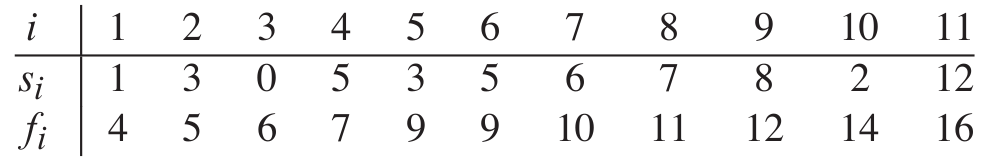
\includegraphics[width=0.7\textwidth]{figs/chap05/activity-example}
\end{figure}
\end{itemize}
\end{frame}

\begin{frame}{‌مسئله انتخاب فعالیت‌ها}
\begin{itemize}\itemr
\item[-]
در مثال زیر این نمونه از مسئله انتخاب فعالیت توسط الگوریتم حریصانه بازگشتی حل شده است.
\begin{figure}
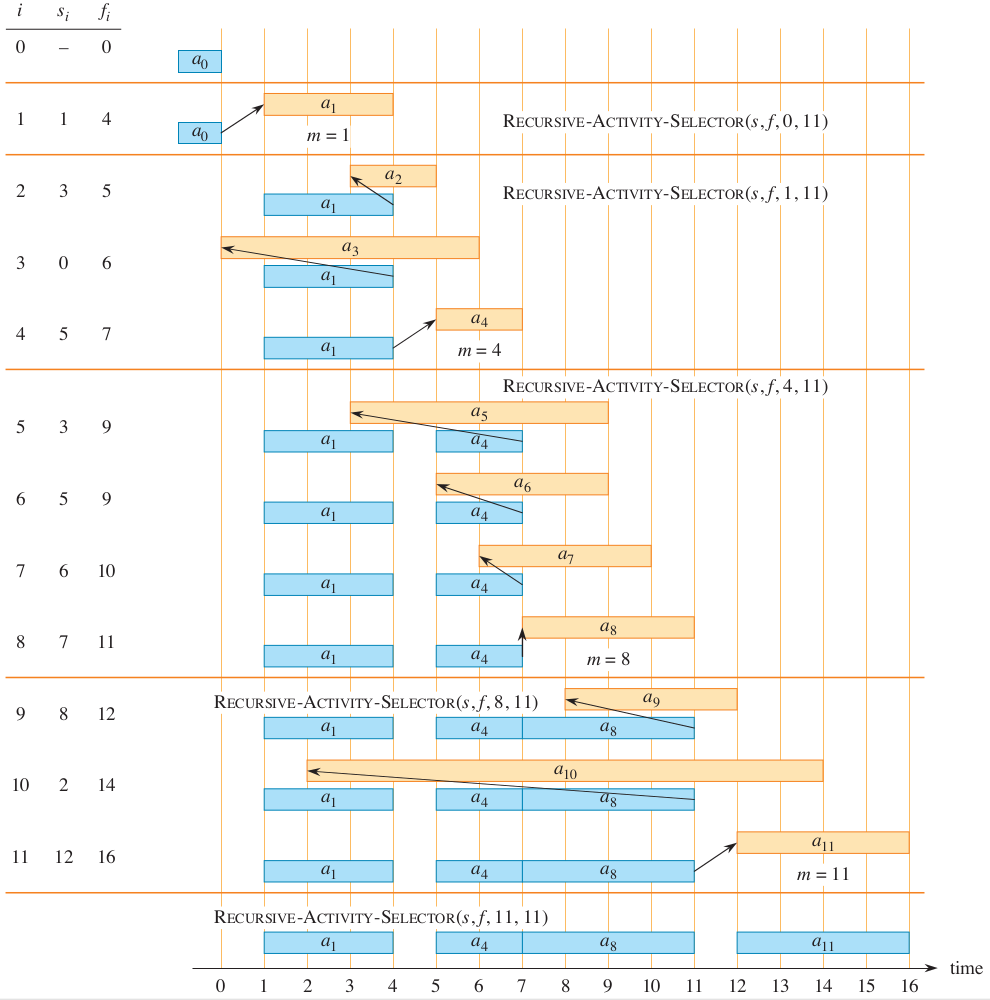
\includegraphics[width=0.47\textwidth]{figs/chap05/activity-recursive-example}
\end{figure}
\end{itemize}
\end{frame}


\iffalse
\begin{frame}{‌مسئله انتخاب فعالیت‌ها}
\begin{itemize}\itemr
\item[-]
این الگوریتم بازگشتی را می‌توانیم به یک الگوریتم غیربازگشتی با یک حلقه تکرار تبدیل کنیم.
\item[-]
به طور کلی همهٔ الگوریتم‌هایی که با یک فراخوانی بازگشتی پایان می‌یابند می‌توانند به الگوریتم‌های غیر بازگشتی با حلقه تکرار تبدیل شوند.
\end{itemize}
\end{frame}
\fi

\begin{frame}{‌مسئله انتخاب فعالیت‌ها}
\begin{itemize}\itemr
\item[-]
الگوریتم زیر مسئله انتخاب فعالیت را به صورت غیر بازگشتی حل می‌کند.
\begin{algorithm}[H]\alglr
  \caption{Greedy-Activity-Selector} 
  \begin{algorithmic}[1]
   \Func{Greedy-Activity-Selector}{s, f, n}
   \State A = \{a[1]\}
   \State k = 1
   \For{m = 2 \To n}
   		\If{s[m] >= f[k]} \LeftComment{is a[m] in S[k] ?}
   				\State A = A $\cup$ \{a[m]\} \LeftComment{yes, so choose it}
   				\State k = m \LeftComment{and continue from there}
   		\EndIf
   	\EndFor
    \State \Return A                       
  \end{algorithmic}
  \label{alg:merge}
\end{algorithm}
\end{itemize}
\end{frame}

\begin{frame}{مسئلهٔ کوله‌پشتی}
\begin{itemize}\itemr
\item[-]
یک الگوریتم حریصانه در هر مرحله انتخابی انجام می‌دهد که در لحظه بهترین انتخاب است و در پایان جواب بهینه نهایی مسئله از این انتخاب‌های بهینه تشکیل شده است. این رویکرد همیشه به جواب بهینه نمی‌رسد اما در برخی مسائل مانند مسئله انتخاب فعالیت جواب بهینه را پیدا می‌کند.
\item[-]
برای حل یک مسئله به روش حریصانه ابتدا ساختار مسئله مشخص می‌شود و یک جواب بازگشتی برای مسئله بر اساس زیر مسئله‌ها طراحی می‌شود. برخلاف روش برنامه‌ریزی پویا که در آن جواب یک مسئله به چند زیرمسئله بستگی پیدا می کند، در مسئله‌هایی که با روش حریصانه حل می‌شوند، جواب یک مسئله به یک زیر مسئله بستگی دارد. پس از یافتن چنین رابطهٔ بازگشتی که در آن جواب یک مسئله تنها به یک زیرمسئله بستگی دارد، یک الگوریتم بازگشتی حریصانه برای مسئله پیدا می‌شود.
%سپس می‌توان الگوریتم بازگشتی را به یک الگوریتم غیر بازگشتی با یک حلقه تکرار تبدیل کرد.
%\item[-]
%به طور خلاصه برای حل یک مسئله به روش حریصانه می‌توان الگوریتمی طراحی کرد که در هر گام یک انتخاب بهینه انجام دهد و تنها یک زیرمسئله برای حل‌کردن باقی می‌ماندو که به طور بازگشتی زیر مسئله‌ها نیز یک انتخاب بهینه صورت می‌دهند. سپس باید اثبات کرد که این روش بهینه را به دست می‌دهد.
\end{itemize}
\end{frame}

\begin{frame}{مسئلهٔ کوله‌پشتی}
\begin{itemize}\itemr
\item[-]
الگوریتم حریصانه مسئله را به صورت از بالا به پایین حل می‌کند، اما برنامه‌ریزی پویا مسئله را از پایین به بالا حل می‌کند.
\item[-]
الگوریتم حریصانه در هر گام انتخابی انجام می‌دهد که بهترین انتخاب است و جواب بهینه از این انتخاب‌های بهینه تشکیل شده است.
\item[-]
در مسئله‌هایی که با الگوریتم حریصانه حل می‌شوند جواب مسئله تنها به جواب یک زیرمسئله بستگی دارد، در حالی که در برنامه‌ریزی پویا، مسئله به چند زیرمسئله بستگی دارد.
\end{itemize}
\end{frame}

\begin{frame}{مسئلهٔ کوله‌پشتی}
\begin{itemize}\itemr
\item[-]
از آنجایی که الگوریتم حریصانه و برنامه‌ریزی پویا شباهت زیادی به یکدیگر دارند و هر دو از زیر مسئله‌های بهینه برای یافتن جواب بهینه مسئله استفاده می‌کنند، ممکن است گاهی برای مسائلی که به روش حریصانه حل می‌شوند، از برنامه‌ریزی پویا استفاده کنیم و یا گاهی به خطا ممکن است بخواهیم مسئله‌ای که به روش برنامه‌ریزی پویا حل می‌شود را به روش حریصانه حل کنیم.
\end{itemize}
\end{frame}


\begin{frame}{مسئلهٔ کوله‌پشتی}
\begin{itemize}\itemr
\item[-]
مسئله کوله پشتی ۱-۰
\fn{1}{\m{0}-\m{1} knapsack problem}
را در نظر بگیرید. یک دزد که مشغول دزدی از یک فروشگاه است، می‌خواهد از بین تعدادی کالا که هر کدام ارزش و وزن مشخصی دارند، تعدادی کالا را در کوله پشتی خود که W کیلوگرم ظرفیت دارد بگذارد، به طوری‌که ارزش کالاهایی که با خود می‌برد حداکثر باشد.
\item[-]
بنابراین این دزد می‌تواند هر زیر مجموعه‌ای از n کالا را بردارد. ارزش کالای i ام برابر است با
\m{v_i}
و وزن آن برابراست با
\m{w_i}
به طوری‌که
\m{v_i}
و
\m{w_i}
دو عدد صحیح هستند. ظرفیت کوله‌پشتی W است و هدف جمع‌آوری تعدادی کالا است که مجموع ارزش آنها حداکثر ممکن باشد.
\item[-]
به این مسئله، مسئله کوله‌پشتی ۱-۰ گفته می‌شود، زیرا دزد به ازای هر کالا باید یا آن را بگذارد یا بردارد و نمی‌تواند قسمتی از کالا را ببرد و قسمتی را بگذارد.
\item[-]
در مسئله کوله پشتی کسری
\fn{2}{fractional knapsack problem}
 دزد می‌تواند یک کالا را به دو قسمت غیر مساوی تقسیم کند و قسمتی از آن را بردارد و قسمتی را با خود ببرد.
\end{itemize}
\end{frame}


\begin{frame}{مسئلهٔ کوله‌پشتی}
\begin{itemize}\itemr
\item[-]
مسئله کوله پشتی ۱-۰ یک مسئلهٔ بهینه‌سازی است که ویژگی آن داشتن زیر ساختار بهینه است، بدین معنی که یک جواب بهینه برای یک مسئله، از جواب بهینه برای زیرمسئله‌های آن تشکیل شده است.
درواقع اگر کالاهای پر ارزش با حداکثر مجموع وزن W را در نظر بگیریم که کالای j را در برگرفته‌اند، آنگاه کالاهای کوله‌پشتی بدون کالای j باید پر ارزش‌ترین کالاها با حداکثر مجموع وزن
\m{W-w_j}
باشند.
\item[-]
همچنین در مسئله کوله‌پشتی کسری، اگر مجموعهٔ پر ارزش‌ترین کالاها با حداکثر وزن W را در نظر بگیریم که مقدار w از کالای j را در برگرفته باشد، آنگاه بقیه کالاهای داخل کوله‌پشتی منهای قسمت w از کالای j با وزن
\m{W-w}
باید پرارزش‌ترین کالاهایی باشند که دزد می‌تواند از بین کالاهای موجود انتخاب کند.
\item[-]
با وجود اینکه این دو مسئله ساختار بسیار مشابهی دارند، روش حریصانه برای مسئله کوله‌پشتی کسری می‌تواند مورد استفاده قرار بگیرد،
در حالی که
 برای مسئله کوله‌پشتی ۱-۰ راه‌حل حریصانه جواب بهینه به دست نمی‌دهد و باید از روش برنامه‌ریزی پویا استفاده کرد.
\end{itemize}
\end{frame}


\begin{frame}{مسئلهٔ کوله‌پشتی}
\begin{itemize}\itemr
\item[-]
برای حل مسئله کوله‌پشتی توسط روش حریصانه، ابتدا ارزش یک کیلوگرم از هر کالا را به صورت
\m{v_i/w_i}
محاسبه می‌کنیم. وقتی ارزش هر کالا مشخص شد، دزد از با ارزش‌ترین کالا شروع می‌کند و سعی می‌کند کوله‌پشتی خود را پر کند. اگر پرارزش‌ترین کالا به اتمام رسید و هنوز کوله‌پشتی فضای خالی داشت، دزد با دومین کالای پرارزش ادامه می‌دهد و سعی می‌کند آنقدر از آن کالا بر دارد تا کوله پشتی پر شود و اگر کوله‌پشتی با کالای پرارزش دوم پر نشد به سراغ کالای پرارزش سوم می‌رود. این روند آنقدر ادامه پیدا می‌کند تا کوله‌پشتی پر شود. این الگوریتم حریصانه نیاز به مرتب‌سازی کالاها بر اساس ارزش آنها در واحد وزن دارد که این کار با استفاده از یک الگوریتم مرتب‌سازی سریع در زمان
\m{O(n \lg n)}
برای 
\m{n}
کالا انجام می‌شود.
\end{itemize}
\end{frame}

\begin{frame}{مسئلهٔ کوله‌پشتی}
\begin{itemize}\itemr
\item[-]
برای اینکه در مسئلهٔ کوله‌پشتی کسری از الگوریتم توصیف شده استفاده کنیم، باید اثبات کنیم الگوریتم درست است.
\item[-]
می‌توانیم درستی این الگوریتم را با استفاده از برهان خلف ثابت کنیم.
فرض کنید کالاهای برداشته شده در کوله‌پشتی بهینه، شامل کالای m که بیشترین چگالی ارزشی
\fn{1}{value density}
 را دارد نشود. به عبارت دیگر کالای m که چگالی ارزشی آن
\m{v_m / w_m}
است به طوری که
\m{\forall i, v_m / w_m > v_i/w_i}
در کوله‌پشتی بهینه نباشد.
دقت کنید که در مسئلهٔ کوله‌پشتی کسری، الزاما کوله‌پشتی پر می‌شود.
\item[-]
بنابراین در کوله‌پشتی کالای k وجود دارد که چگالی ارزشی آن از کالای m کمتر است، یعنی
\m{v_k/w_k < v_m/w_m} .
در اینصورت می‌توانیم x کیلوگرم از کالای k را از کوله‌پشتی برداریم و x کیلوگرم از کالای m را در کوله‌پشتی قرار دهیم.
\item[-]
مقدار
\m{x \cdot (v_m/w_m) - x \cdot (v_k/w_k)}
مثبت است، که با فرض اولیه مبنی بر اینکه کوله‌پشتی بهینه است در تناقض دارد، پس کوله‌پشتی الزاما حاوی کالایی با بیشترین چگالی ارزشی است.
\end{itemize}
\end{frame}


\begin{frame}{مسئلهٔ کوله‌پشتی}
\begin{itemize}\itemr
\item[-]
 الگوریتم حریصانه برای مسئله کوله‌پشتی ۱-۰ نمی‌تواند مورد استفاده قرار بگیرد.
\item[-]
در مسئله کوله‌پشتی ۱-۰ زیر مسئله‌ها باید با یکدیگر مقایسه شوند، در صورتی که جواب بهینه مسئله کوله پشتی کسری تنها به یک زیر مسئله بستگی دارد.
\item[-]
می‌توان با استفاده از یک مثال نقض نشان داد که الگوریتم حریصانه نمی‌تواند در کوله‌پشتی ۱-۰ مورد استفاده قرار بگیرد.
\end{itemize}
\end{frame}


\begin{frame}{مسئلهٔ کوله‌پشتی}
\begin{itemize}\itemr
\item[-]
مثال زیر نشان می‌دهد که روش حریصانه برای مسئله کوله پشتی ۱-۰ الزاما جواب بهینه را به دست نمی‌آورد. با وجود اینکه کالای اول پر ارزش‌ترین کالاست ولی در مسئله کوله پشتی ۱-۰ در جواب بهینه انتخاب نمی‌شود.
 \begin{figure}
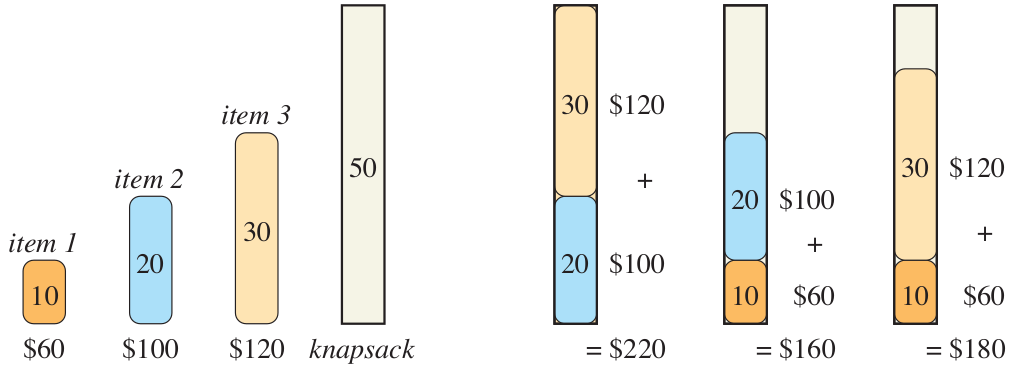
\includegraphics[width=0.7\textwidth]{figs/chap05/knapsack-example}
 \end{figure}
\item[-]
همچنین اگر پر کردن کوله پشتی را با کالاهایی آغاز کنیم که بیشترین قیمت را دارند،
ممکن است کالاها با قیمت بالا حجم زیادی را اشغال کرده و کوله پشتی را پر کنند، در صورتی که مجموع ارزش کالاهای کم ارزش‌تر بیشتر باشد.
\end{itemize}
 \end{frame}


\begin{frame}{مسئلهٔ کوله‌پشتی}
\begin{itemize}\itemr
\item[-]
در مسئله کوله پشتی کسری توسط یک الگوریتم حریصانه شروع به پر کردن کوله پشتی توسط پرارزش‌ترین کالاها می‌کنیم.
\begin{figure}
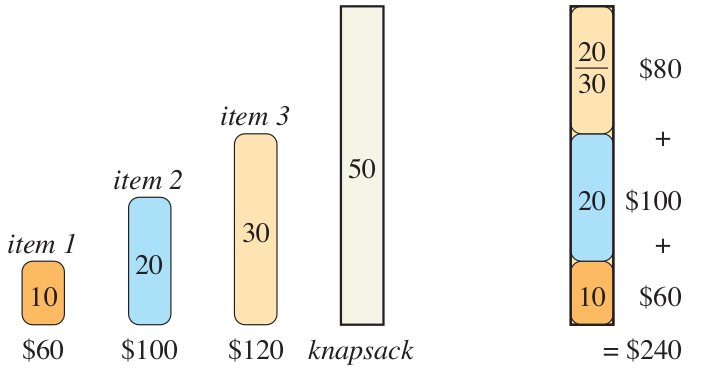
\includegraphics[width=0.6\textwidth]{figs/chap05/knapsack-greedy}
\end{figure}
\end{itemize}
\end{frame}




\begin{frame}{‌کدهای هافمن}
\begin{itemize}\itemr
\item[-]
کدهای هافمن
\fn{1}{Huffman codes}
برای فشرده‌سازی داده‌ها استفاده می‌شوند. این کدها بسته به ویژگی داده‌ها، می‌توانند بین ۲۰ تا ۹۰ درصد در میزان حافظه مورد نیاز برای ذخیره‌سازی داده‌ها صرفه جویی کنند.
\item[-]
 الگوریتم حریصانه هافمن جدولی شامل تعداد تکرار حروف دریافت کرده، سپس برای هر حرف یک کد تولید می‌کند، به طوری که ذخیرهٔ یک متن با استفاده از کدهای تولید شده کمترین میزان حافظه را اشغال کند.
\item[-]
فرض کنید یک فایل داده‌ای داریم که شامل
۱۰۰،۰۰۰
حرف (کاراکتر) است و می‌خواهیم فایل را به صورت فشرده ذخیره کنیم و همچنین می‌دانیم ۶ حرف اول الفبا دارای تعداد تکرارهای ذکر شده در جدول زیر هستند.
\begin{figure}
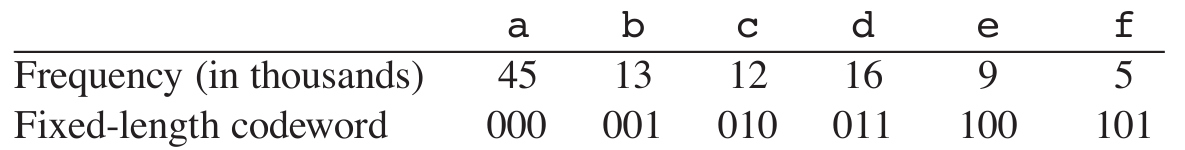
\includegraphics[width=0.7\textwidth]{figs/chap05/huffman-example}
\end{figure}
\end{itemize}
\end{frame}


\begin{frame}{‌کدهای هافمن}
\begin{itemize}\itemr
\item[-]
برای مثال حرف a در این فایل
۴۵،۰۰۰
بار و حرف b تعداد
۱۳،۰۰۰
بار تکرار شده‌اند.
\item[-]
برای نمایش داده‌ها در این فایل راه‌های زیادی وجود دارد. در اینجا از یک کد گذاری دودویی استفاده می‌کنیم. به ازای هر یک از حروف الفبا یک عدد دودویی در نظر گرفته و آن حرف را با کد در نظر گرفته شده نمایش می‌دهیم. به این کدهای دودویی
\fn{1}{binary character  code}
،به اختصار کد می‌گوییم.
\item[-]
می‌توانیم از کدهایی با طول ثابت
\fn{2}{fixed-length code}
استفاده کنیم، که در اینصورت به تعداد
\m{ \lceil \lg n \rceil}
بیت برای نمایش n حرف نیاز داریم. برای ۶ حرف به ۳ بیت نیاز داریم :
\m{a = 000}،
\m{b = 001}،
\m{c = 010}،
\m{d = 011}،
\m{e = 100}و
\m{f = 101}.
\item[-]
با استفاده از این روش کد گذاری برای یک فایل شامل
۱۰۰،۰۰۰
حرف به
۳۰۰،۰۰۰
بیت نیاز داریم. اما آیا می‌توانیم با تعداد کمتری بیت این فایل را ذخیره کنیم؟
\end{itemize}
\end{frame}


\begin{frame}{‌کدهای هافمن}
\begin{itemize}\itemr
\item[-]
برای فشرده‌سازی این فایل متنی و ذخیره‌سازی حروف به طور کارامدتر از کدهایی با طول متغیر
\fn{1}{variable-length code}
استفاده می‌کنیم.
\item[-]
برای نمایش حروفی که تعداد تکرار بیشتری دارند، از کدهای کوتاه‌تر و برای نمایش حروفی که تعداد تکرار کمتری دارند، از کدهای بلندتر استفاده می‌کنیم.
\end{itemize}
\end{frame}


\begin{frame}{‌کدهای هافمن}
\begin{itemize}\itemr
\item[-]
برای مثال یک روش کدگذاری با کدهای طول متغیر در شکل زیر نمایش داده شده است.
\begin{figure}
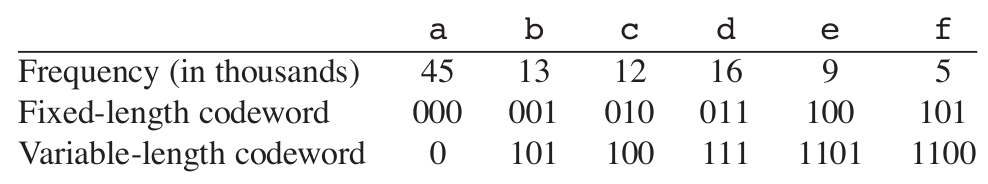
\includegraphics[width=0.7\textwidth]{figs/chap05/huffman-vlc}
\end{figure}
\item[-]
در اینجا از بیت صفر برای نمایش a و عدد چهاربیتی
۱۱۰۰
برای نمایش حروف f استفاده می‌کنیم.
\item[-]
برای نمایش یک فایل شامل
۱۰۰،۰۰۰
حرف با تعداد‌های تکرار ذکر شده به تعداد بیت زیر نیاز داریم‌ :
\begin{align*}
\m{(45 \times 1 + 13 \times 3 + 12 \times 3 + 16 \times 3 + 9 \times 4 + 5 \times 4) \times 1000 = 224000~~\text{bit} }
\end{align*}
\item[-]
بنابراین با استفاده از این روش کدگذاری توانستیم به جای ۳۰۰ هزار بیت از ۲۲۴ هزار بیت استفاده کنیم و حدود ۲۵ درصد در فضای حافظهٔ مورد نیاز صرفه‌جویی کنیم.
\end{itemize}
\end{frame}


\begin{frame}{‌کدهای هافمن}
\begin{itemize}\itemr
\item[-]
در روش کدگذاری استفاده شده، هیچ‌یک از کدها پیشوند کدهای دیگر نبودند. بدین ترتیب به افزودن خط فاصله بین کدها نیازی نداریم و می‌توانیم کدهای یکتا را شناسایی کنیم. به این مجموعهٔ کد، کدهای بدون پیشوند
\fn{1}{prefix-free code}
می‌گوییم.
\item[-]
ثابت شده‌است که کدهای بدون پیشوند بهینه‌ترین روش برای فشرده‌سازی اطلاعات است و هیچ روش کدگذاری بهینه‌تری برای فشرده‌سازی بیشتر وجود ندارد.
\item[-]
با استفاده از روش کدگذاری می‌توانیم کلمهٔ face را به صورت
\begin{align*}
\m{1100 \cdot 0 \cdot 100 \cdot 1101 = 110001001101}
\end{align*}
ذخیره کنیم. در اینجا عملگر
\m{" \cdot "}
به معنی الحاق دو رشته است.
\end{itemize}
\end{frame}


\begin{frame}{‌کدهای هافمن}
\begin{itemize}\itemr
\item[-]
کدهای بدون پیشوند فرایند کدگشایی را ساده می‌کنند. از آنجایی که هیچ کدی پیشوند کد دیگری نیست، کدگذاری یک فایل ابهام ایجاد نمی‌کند. برای کدگشایی یک فایل از ابتدای فایل شروع می‌کنیم و کدها را به ترتیب تبدیل به حروف می‌کنیم.
\item[-]
برای مثال در کدگشایی رشتهٔ
\m{100011001101}
کد
\m{1}
یا
\m{10}
یا
\m{1000}
وجود ندارند و تنها کدی که می‌توان در ابتدای این رشته تشخیص داد، کد
\m{100}
است. این کد معادل کلمه
cafe
می‌باشد.
\begin{align*}
\m{100011001101 = 100 \cdot 0 \cdot 1100 \cdot 1101 = cafe}
\end{align*}
\begin{figure}
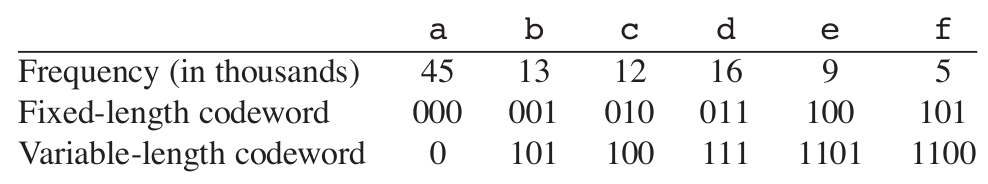
\includegraphics[width=0.7\textwidth]{figs/chap05/huffman-vlc}
\end{figure}
\end{itemize}
\end{frame}


\begin{frame}{‌کدهای هافمن}
\begin{itemize}\itemr
\item[-]
در فرایند کدگشایی برای جستجوی بهینهٔ کدها و حروف متناظر آنها از یک درخت دودویی استفاده می‌کنیم. برگ‌های این درخت دودویی، حروف متناظر با کدهایی هستند که از الحاق کدهای روی یال‌ها از ریشه تا برگ مورد نظر به دست می‌آیند.
\item[-]
به عبارت دیگر کد مربوط به یک حرف درواقع یک مسیر از ریشه تا حرف مورد نظر است به طوری‌که صفر به معنای رفتن به سمت فرزند سمت چپ و یک به معنای رفتن به فرزند سمت راست است.
\end{itemize}
\end{frame}


\begin{frame}{‌کدهای هافمن}
\begin{itemize}\itemr
\item[-]
شکل‌های زیر دو درخت متفاوت برای کدگذاری حروف را نشان می‌دهند.
\begin{figure}
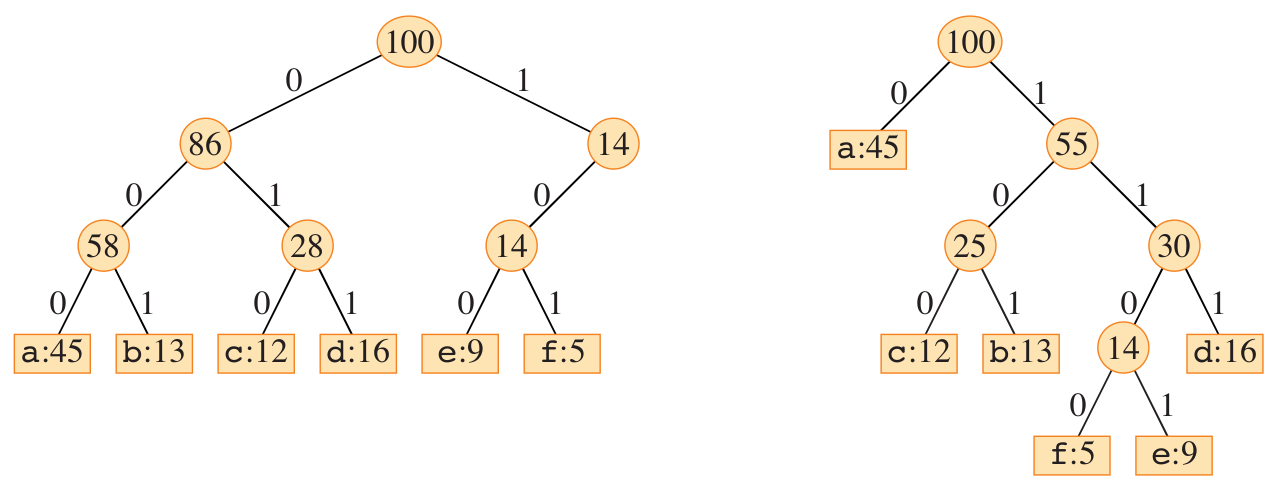
\includegraphics[width=0.9\textwidth]{figs/chap05/huffman-tree}
\end{figure}
\end{itemize}
\end{frame}


\begin{frame}{‌کدهای هافمن}
\begin{itemize}\itemr
\item[-]
می‌توان ثابت کرد که یک کدگذاری بهینه همیشه توسط یک درخت دودویی پُر
\fn{1}{full binary tree}
(درخت اکیدا دودویی)
نشان داده می‌شود،
بدین معنی که هر رأس میانی در درخت بهینه الزاما دارای دو فرزند است. در شکل زیر در سمت چپ، درخت دودویی پر نیست، زیرا به ازای کد ۱۱ هیچ حرفی وجود ندارد،
پس کدگذاری توسط این درخت نمی‌تواند یک کدگذاری بهینه باشد،
 اما درخت سمت راست یک درخت دودویی پر را نشان می‌دهد.
\begin{figure}
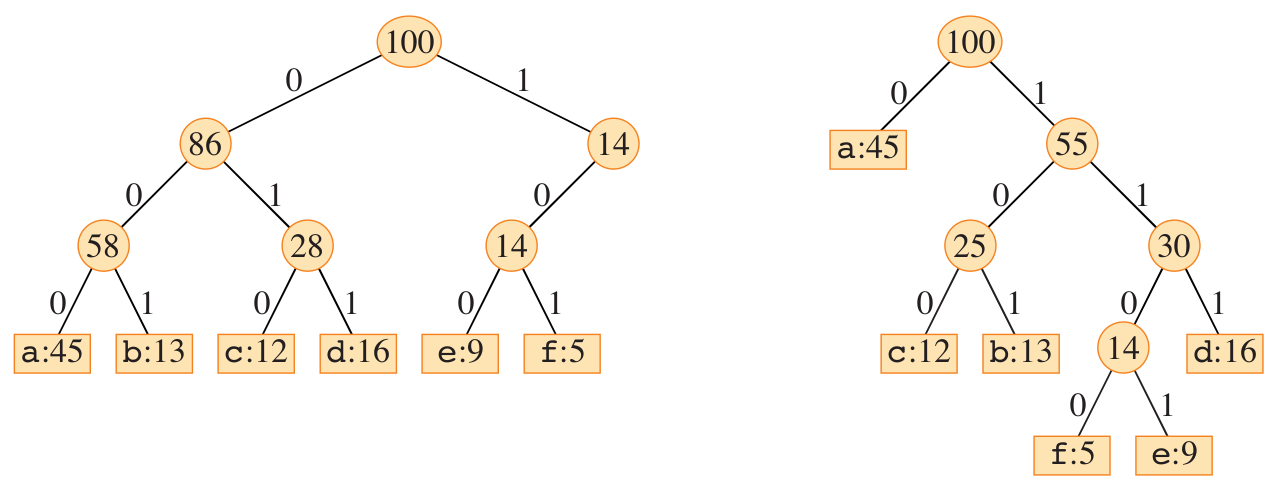
\includegraphics[width=0.6\textwidth]{figs/chap05/huffman-tree}
\end{figure}
%\item[-]
%در درخت سمت چپ از کد ۱ برای هیچ حرفی استفاده نشده است و به همین دلیل این کدگذاری نمی‌تواند بهینه باشد.
\end{itemize}
\end{frame}


\begin{frame}{‌کدهای هافمن}
\begin{itemize}\itemr
\item[-]
یک درخت دودویی پر با 
\m{n}
 برگ الزاما 
\m{n-1}
رأس غیربرگ دارد.
\item[-]
اگر
\m{C}
الفبای مورد نظر برای کدگذاری باشد، درختی که برای کدهای بدون پیشوند بهینه به دست می‌آید، دارای
\m{|C|}
برگ است که هر برگ متناظر با یک حرف است و تعداد
\m{|C| - 1}
رأس میانی (غیربرگ) در درخت داریم.
\end{itemize}
\end{frame}


\begin{frame}{‌کدهای هافمن}
\begin{itemize}\itemr
\item[-]
اگر درخت
\m{T}
درختی برای کدهای بدون پیشوند باشد، می‌توانیم تعداد بیت‌های مورد نیاز برای کدگذاری یک فایل را محاسبه کنیم. به ازای هر حرف c در الفبای
\m{C}
 ، فرض کنید
\m{c.freq}
تعداد تکرار آن حرف در فایل باشد و فرض کنید
\m{d_T(c)}
عمق برگ متناظر با حرف c در درخت باشد. دقت کنید که
\m{d_T(c)}
طول کد متناظر با حرف c نیز هست. در اینصورت تعداد بیت‌های مورد نیاز برای کدگذاری فایل داده‌ای برابراست با
\begin{align*}
\m{B(T) = \sum_{c \in C} c.freq \times d_T(c)}
\end{align*}
\item[-]
به مقدار
\m{B(T)}
هزینه
\fn{1}{cost}
درخت T می‌گوییم.
\end{itemize}
\end{frame}


\begin{frame}{‌کدهای هافمن}
\begin{itemize}\itemr
\item[-]
هافمن یک الگوریتم حریصانه ابداع کرد که کدهای بدون پیشوند بهینه تولید می‌کند. این کدها به کدهای هافمن مشهور هستند.
%\item[-]
%ابتدا الگوریتم حریصانهٔ تولید کدهای هافمن را توضیح می‌دهیم و سپس اثبات می‌کنیم چرا الگوریتم حریصانه در اینجا می‌تواند مورد استفاده قرار بگیرد.
\item[-]
ورودی الگوریتم هافمن مجموعهٔ
\m{C}
شامل n حرف است، به طوری که هر عضو
\m{c \in C}
یک حرف است که ویژگی
\m{c.freq}
تعداد تکرار آن را نشان می‌دهد.
\item[-]
این الگوریتم درخت T را برای تولید کدهای بهینه می‌سازد. این درخت از پایین به بالا تولید می‌شود، بدین معنی که الگوریتم با
\m{|C|}
برگ آغاز می‌کند و با ادغام این برگ‌ها به صورت ساختار درختی، کل درخت را تا ریشه می‌سازد.
\item[-]
در این الگوریتم از یک صف اولویت استفاده می‌شود که حروف با کمترین تعداد‌های تکرار به ترتیب از صف خارج می‌شوند.
\end{itemize}
\end{frame}


\begin{frame}{‌کدهای هافمن}
\begin{itemize}\itemr
\item[-]
الگوریتم هافمن به صورت زیر است.
\begin{algorithm}[H]\alglr
  \caption{Huffman} 
  \begin{algorithmic}[1]
   \Func{Huffman}{C}
   \State n = |C|
   \State Q = C
   \For{i = 1 \To n - 1}
   			\State allocate a new node z
   			\State x = Extract-Min(Q)
   			\State y = Extract-Min(Q)
   			\State z.left = x
   			\State z.right = y
   			\State z.freq = x.freq + y.freq
   			\State Insert(Q,z)
   	\EndFor
   	\State \Return Extract-Min(Q) \LeftComment{the root of the tree is the only node left}                       
  \end{algorithmic}
  \label{alg:merge}
\end{algorithm}
\end{itemize}
\end{frame}


\begin{frame}{‌کدهای هافمن}
\begin{itemize}\itemr
\item[-]
برای مثالی که در قبل مطرح کردیم، الگوریتم هافمن به صورت زیر عمل می‌کند.
\begin{figure}
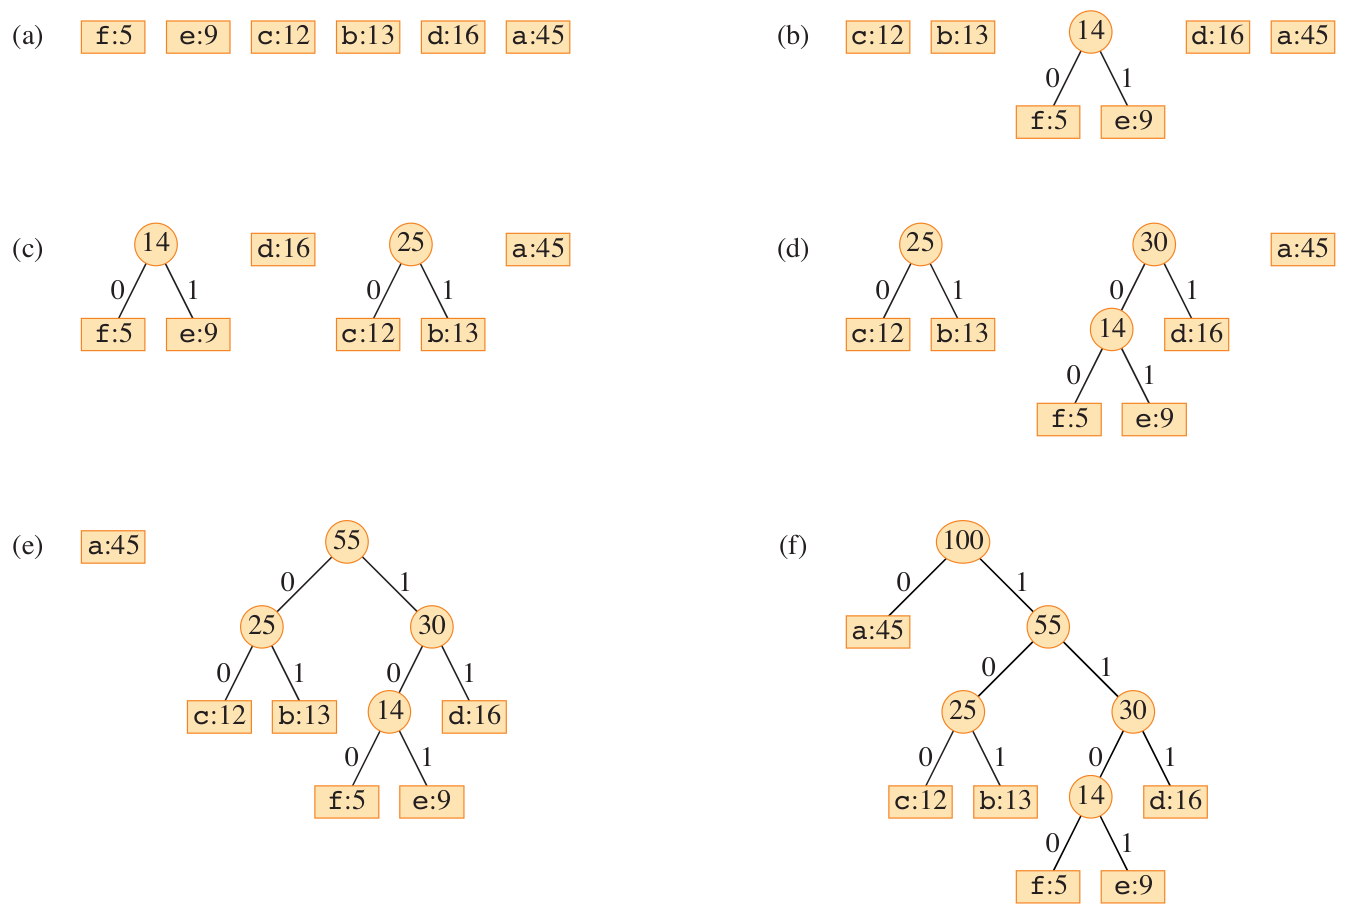
\includegraphics[width=0.7\textwidth]{figs/chap05/huffman-alg-ex}
\end{figure}
\end{itemize}
\end{frame}


\begin{frame}{‌کدهای هافمن}
\begin{itemize}\itemr
\item[-]
زمان الگوریتم هافمن به نحوهٔ پیاده‌سازی صف اولویت بستگی دارد. فرض کنیم با بهینه‌ترین الگوریتم موجود، صف اولویت برای یک الفبا با n حرف در زمان
\m{O(n)}
ساخته می‌شود.
\item[-]
حلقهٔ اصلی در الگوریتم هافمن
\m{n-1}
بار تکرار می‌شود، زیرا تعداد رئوس غیربرگ
\m{n-1}
است
 و از آنجایی که در هر بار استفاده از صف اولویت به زمان
\m{\lg n}
نیاز داریم، بنابراین زمان اجرای الگوریتم
\m{O(n \lg n)}
است.
\item[-]
بنابراین کل زمان اجرای الگوریتم هافمن برای الفبای n حرفی برابراست با
\m{O(n \lg n)}.
\end{itemize}
\end{frame}


\begin{frame}{‌کدهای هافمن}
\begin{itemize}\itemr
\item[-]
برای اثبات اینکه الگوریتم حریصانه هافمن درست است، نشان می‌دهیم مسئله تعیین کدهای بدون پیشوند بهینه دارای ویژگی انتخاب حریصانه است.
\item[-]
به عبارت دیگر می‌خواهیم اثبات کنیم دو رأس با کمترین تعداد تکرار الزاما در درخت کدهای بهینه همزاد یکدیگرند و در بیشترین عمق قرار می‌گیرند.
\end{itemize}
\end{frame}


\begin{frame}{‌کدهای هافمن}
\begin{itemize}\itemr
\item[-]
قضیه : فرض کنید
\m{C}
یک الفبا باشد به طوری‌که
\m{c \in C}
دارای تعداد تکرار
\m{c.freq}
باشد. فرض کنید x و y دو حرف در C با کمترین تعداد‌های تکرار باشند. آنگاه یک کدگذاری بدون پیشوند بهینه برای C وجود دارد به طوری‌که x و y طول یکسانی دارند و تنها در بیت آخر متفات‌اند، یعنی همزاد یکدیگرند و همچنین در بیشترین عمق درخت قرار دارند.
\end{itemize}
\end{frame}


\begin{frame}{‌کدهای هافمن}
\begin{itemize}\itemr
\item[-]
اثبات : ایدهٔ اثبات این است که درخت
\m{T}
که یک درخت بهینهٔ بدون پیشوند را در نظر بگیریم و آن را تغییر دهیم تا یک درخت دودویی بدون پیشوند دیگر ساخته شود به طوری‌که در درخت ساخته شده x و y همزاد
\fn{1}{sibiling}
و در عمق بیشینه در درخت
\m{T}
باشند. چنین درختی که در آن x و y همزاد یکدیگرند یعنی طول یکسان دارند و تنها در بیت آخر متفاوت‌اند، نیز یک درخت بهینه خواهد بود.
\item[-]
فرض کنید a و b دو حرف باشند که در درخت
\m{T}
همزاد هستند و در بیشترین عمق درخت قرار دارند. حال فرض کنید
\m{a.freq \leqslant b.freq}
و
\m{x.freq \leqslant y.freq}.
از آنجایی‌که
\m{x.freq}
و
\m{y.freq}
کمترین تعداد‌های تکرار هستند و
\m{a.freq}
و
\m{b.freq}
دو تعداد تکرار دلخواه هستند، بنابراین خواهیم داشت
\m{x.freq \leqslant a.freq}
و
\m{y.freq \leqslant b.freq}.
\item[-]
بنابراین می‌توانیم داشته باشیم
\m{x.freq = a.freq}
و
\m{y.freq = b.freq}
که در اینصورت قضیه به طور بدیهی درست است، زیرا a و b دارای کمترین تعداد تکرار هستند.
 پس فرض می‌کنیم تعداد تکرارهای
 x 
 و
 y
 متفاوت از a و b هستند.
\end{itemize}
\end{frame}


\begin{frame}{‌کدهای هافمن}
\begin{itemize}\itemr
\item[-]
همانطور که شکل زیر نشان می‌دهد، فرض کنید جای a و x را در درخت
\m{T}
عوض می‌کنیم و درخت
\m{T'}
را به‌دست می‌آوریم و جای b و y را در درخت 
\m{T'}
عوض کرده،
درخت
\m{T''}
را به دست می‌آوریم.
\begin{figure}
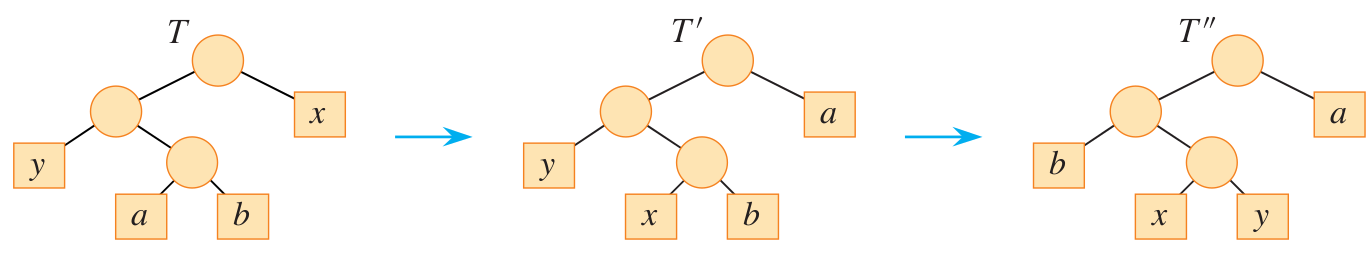
\includegraphics[width=0.9\textwidth]{figs/chap05/huffman-proof}
\end{figure}
\item[-]
نشان می‌دهیم که هزینهٔ درخت
\m{T''}
کوچکتر یا مساوی درخت
\m{T}
 است.
 از آنجایی که فرض کردیم درخت 
 \m{T}
 یک درخت بهینه است، بنابراین هزینه درخت 
 \m{T''}
 و
\m{T}
باید برابر باشد.
\end{itemize}
\end{frame}


\begin{frame}{‌کدهای هافمن}
\begin{itemize}\itemr
\item[-]
تفاوت هزینهٔ درخت
\m{T}
و
\m{T'}
به صورت زیر خواهد بود.
\begin{align*}
\m{B(T)} & \m{- B(T')}\\
&\m{= \sum_{c \in C} c.freq \cdot d_T(c) - \sum_{c \in C} c.freq \cdot d_{T'}(c)}\\
&\m{= x.freq \cdot d_T(x) + a.freq \cdot d_T(a) - x.freq \cdot d_{T'}(x) - a.freq \cdot d_{T'}(a)}\\
&\m{= x.freq \cdot d_T(x) + a.freq \cdot d_T(a) - x.freq \cdot d_T(a) - a.freq \cdot d_T(x)}\\
&\m{= (a.freq - x.freq) (d_T(a) - d_T(x))}\\
&\m{\geqslant 0}
\end{align*}
\end{itemize}
\end{frame}


\begin{frame}{‌کدهای هافمن}
\begin{itemize}\itemr
\item[-]
از آنجایی که
\m{a.freq - x.freq}
و همچنین
\m{d_T(a) - d_T(x)}
غیر منفی هستند، بنابراین مقدار
\m{B(T) - B(T')}
مثبت است.
\item[-]
درواقع
\m{a.freq - x.freq}
غیر منفی است زیرا x یک برگ با حداقل تعداد تکرار است و
\m{d_T(a) - d_T(x)}
غیر منفی است زیرا a یک برگ با عمق بیشینه در درخت
\m{T}
است.
\item[-]
به همین ترتیب تعویض y و b هزینه را افزایش نمی‌دهد و بنابراین
\m{B(T') - B(T'')}
نیز غیر منفی است.
\item[-]
بنابراین
\m{B(T'') \leqslant B(T') \leqslant B(T)}
و چون
\m{T}
بهینه است بنابراین داریم
\m{B(T) \leqslant B(T'')}
و بنابراین
\m{B(T'') = B(T)}
در نتیجه
\m{T''}
یک درخت بهینه است که در آن x و y دو برگ همزاد با عمق حداکثر هستند و قضیه ثابت می‌شود.
\end{itemize}
\end{frame}


\begin{frame}{‌کدهای هافمن}
\begin{itemize}\itemr
\item[-]
این قضیه در واقع نشان می‌دهد که ساختن درخت بهینه، می‌تواند با انتخاب حریصانه ادغام دو حرف با کمترین تعداد تکرار آغاز شود و ادامه یابد. بنابراین از بین همهٔ انتخاب‌ها برای ادغام الگوریتم هافمن دو حرف با کمترین تعداد را در هر مرحله انتخاب می‌کند که یک انتخاب بهینه است، و همچنین درخت کلی به دست آمده در نهایت یک درخت بهینه خوهد بود.
\end{itemize}
\end{frame}


\begin{frame}{‌کدهای هافمن}
\begin{itemize}\itemr
\item[-]
حال می‌خواهیم ثابت کنیم ساختن کدهای بدون پیشوند بهینه دارای ویژگی زیر ساختار بهینه است.
\item[-]
به عبارت دیگر، می‌خواهیم اثبات کنیم اگر رأس z به عنوان پدر رئوس x و y با کمترین تعداد تکرار به همراه بقیه رئوس درخت به جز x و y ، یک درخت کدهای بهینه را تشکیل دهند، آنگاه درختی که در آن x و y به عنوان فرزندان z اضافه شده‌اند نیز درخت کدهای بهینه است.
\end{itemize}
\end{frame}


\begin{frame}{‌کدهای هافمن}
\begin{itemize}\itemr
\item[-]
قضیه : فرض کنید
\m{C}
یک الفبا باشد به طوری‌که برای هر حرف
\m{c \in C}
تعداد تکرار c برابر با
\m{c.freq}
باشد. فرض کنید x و y دو حرف در
\m{C}
با تعداد تکرار حداقل باشند. فرض کنید
\m{C'}
همان الفبای 
\m{C}
 باشد به طوری‌که حروف x و y حذف شده و حرف z به آن اضافه شده است، بنابراین
\m{C' = (C - \{x,y\}) \cup \{z\}}
تعداد تکرار همهٔ حروف در
\m{C'}
برابر با حروف
\m{C}
هستند و همچنین
\m{z.freq = x.freq + y.freq}.
فرض کنید
\m{T'}
درختی باشد که کدهای بدون پیشوند بهینه
\m{C'}
را نمایش می‌دهد. آنگاه درخت
\m{T}
که از درخت
\m{T'}
به دست آمده و در آن رأس z با یک رأس میانی با دو فرزند x و y به جایگزین شده است، کدهای بدون پیشوند بهینه برای الفبای
\m{C}
را نمایش می‌دهد.
\end{itemize}
\end{frame}


\begin{frame}{‌کدهای هافمن}
\begin{itemize}\itemr
\item[-]
اثبات : ابتدا نشان می‌دهیم چگونه هزینه
\m{B(T)}
از درخت
\m{T}
بر اساس هزینهٔ
\m{B(T')}
از درخت
\m{T'}
بیان می‌شود.
\item[-]
به ازای هر حرف
\m{c \in C - \{x,y\}}
، داریم
\m{d_T(c) = d_{T'}(c)}
و بنابراین
\m{c.freq \times d_T(c) = c.freq \times d_{T'}(c)} .
\item[-]
چون
\m{d_T(x) = d_T(y) = d_{T'}(z) + 1}
،بنابراین داریم :
\begin{align*}
\m{x.freq \times d_T(x) + y.fraq \times d_T(y)} & \m{= (x.freq + y.freq)(d_{T'}(z) + 1)}\\
& \m{= z.freq \times d_{T'}(z) + (x.freq + y.freq)}
\end{align*}
\item[-]
بنابراین نتیجه می‌گیریم
\m{B(T) = B(T') + x.freq + y.freq}
که برابر است با
\m{B(T') = B(T) - x.freq - y.freq}.
\item[-]
حال از برهان خلف استفاده می‌کنیم.
\end{itemize}
\end{frame}


\begin{frame}{‌کدهای هافمن}
\begin{itemize}\itemr
\item[-]
فرض کنید
\m{T}
درخت بهینه بدون پیشوند برای
\m{C}
نیست. بنابراین یک درخت
\m{T''}
بهینه وجود دارد به طوری‌که
\m{B(T'') < B(T)}.
درخت
\m{T''}
دو رأس x و y را به عنوان همزاد درخود دارد.
\item[-]
حال فرض کنید
\m{T'''}
همان درخت
\m{T''}
باشد که در آن پدر مشترک x و y با رأس برگ z جایگزین شده است به طوری‌که
\m{z.freq = x.freq + y.freq}
\item[-]
بنابراین :
\begin{align*}
\m{B(T''')} & \m{= B(T'') - x.freq - y.freq}\\
& \m{< B(T) - x.freq - y.freq}\\
& \m{= B(T')}
\end{align*}
\item[-]
به این نتیجه رسیدیم که 
\m{T'''}
یک درخت بهینه برای 
\m{C'}
است، اما با این نتیجه 
 به تناقض می‌رسیم زیرا فرض کردیم
\m{T'}
درخت بدون پیشوند بهینه برای
\m{C'}
است. بنابراین
\m{T}
باید کدهای بدون پیشوند بهینه برای الفبای
\m{C}
را نمایش دهد.
\end{itemize}
\end{frame}


\begin{frame}{‌کدهای هافمن}
\begin{itemize}\itemr
\item[-]
دو قضیهٔ اثبات شده نشان می‌دهند الگوریتم هافمن کدهای بدون پیشوند بهینه تولید می‌کند.
\end{itemize}
\end{frame}


%%%%%%%%%%%%

%%%%%%%%%%%%
%\section*{References}
%\begin{frame}<0>[noframenumbering]
%\bibliographystyle{apalike}
%\bibliography{docs/bib}
%\end{frame}
%%%%%%%%%%%%

\end{document}
